\section{Background}
\label{sec:background}

Blockchain is a fairly recent technology and can a lot of times be hard to
understand. It leverages cryptographic concepts at its core to make it all
work. In this Section, we will explain some of the key concepts of blockchain
technology and also discuss how wallets work and how they interact with the
blockchain. We will then explore some of the most popular blockchain networks
and token standards, as well as the emerging trend of non-fungible tokens
(NFTs). The Figure \ref{fig:blockchain_concepts} illustrates the most common
concepts of blockchain technology and we'll be mentioning the Wallets (1) in
the Section \ref{subsec:wallets} and what they are for, the Networks (2) in the
Section \ref{subsec:networks} and what differences exist between the most
popular ones, and the Smart Contracts (3) in the Section
\ref{subsec:smart_contracts} and their characteristics.

\begin{figure}[H]
    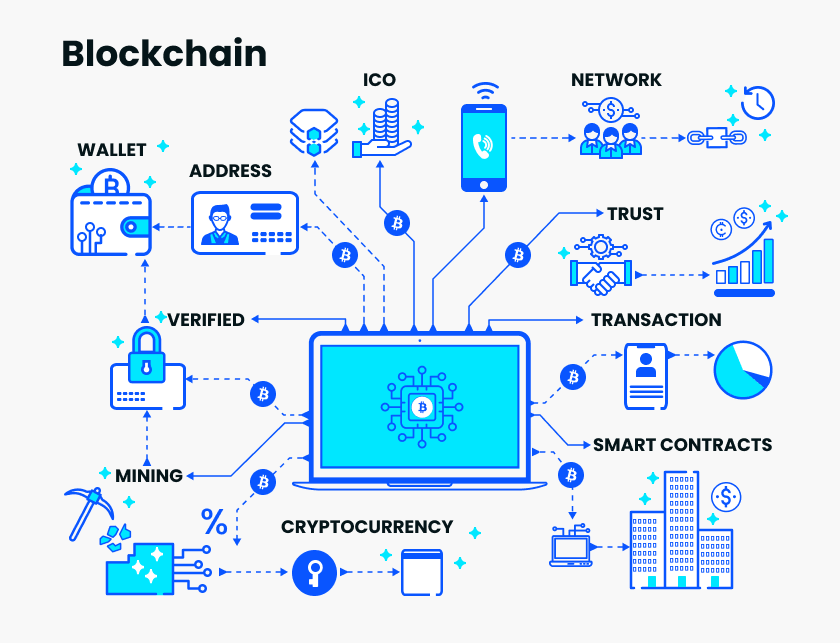
\includegraphics[width=\textwidth*2/3]{Blockchain concepts.png}
    \centering
    \caption[Blockchain concepts]{Blockchain concepts. Adapted from ...}
    \label{fig:blockchain_concepts}
\end{figure}

\subsection{Interacting with the Blockchain}
\label{subsec:interacting_with_the_blockchain}

As we saw, a blockchain works as a decentralized network of nodes, where each
node has a copy of the entire blockchain. This means that in order to interact
with the blockchain, we need to send transactions to the network, which will
then be validated and added to a block by the nodes. To do this, we need to use
a wallet, which is an application that allows users to manage their digital
assets, interact with smart contracts, and send transactions on the blockchain.
Wallets provide a user-friendly interface for accessing the blockchain network,
signing transactions with private keys, and viewing account balances and
transaction history.

The Figure \ref{fig:how_does_a_blockchain_work} shows the steps of what happens
on a transaction on the blockchain. To execute one, we need to sign it with our
private key, which proves that we are the rightful owner of the assets being
transferred. The transaction is then broadcast to the network, where it is
validated by network participants and added to a block. Once the transaction is
confirmed and included in a block, it becomes part of the immutable blockchain
ledger, visible to all participants in the network.

This is the procedure to make a change to the blockchain state, so you always
have to sign the transaction. To read information from it, you don't need to
sign anything, you just need to query the network for the information you want.

\begin{figure}[H]
    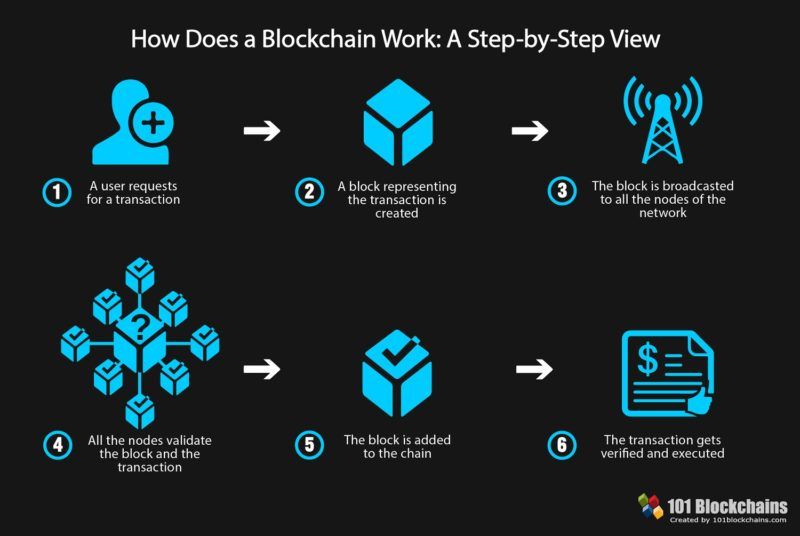
\includegraphics[width=\textwidth*2/3]{How does a blockchain work.jpg}
    \centering
    \caption[How does a blockchain work]{How does a blockchain work. Extracted from ...}
    \label{fig:how_does_a_blockchain_work}
\end{figure}

\subsection{Blockchain}
\label{subsec:blockchain}

So blockchain is a decentralized and distributed ledger technology that enables
the secure recording and sharing of data across a network of computers. At its
core, a blockchain consists of a series of blocks, each containing a list of
transactions. These blocks are linked together in a chronological and immutable
chain, forming a transparent and tamper-proof record of transactions. The key
characteristics of blockchain technology include:

\paragraph{Decentralization:}
Unlike traditional centralized systems where data is stored in a single
location or controlled by a central authority, blockchain operates on a
decentralized network of computers (nodes). Each node maintains a copy of the
entire blockchain, ensuring that there is no single point of failure or
control.

\paragraph{Transparency:}
The data recorded on a blockchain is visible to all participants in the
network. This transparency fosters trust among users, as they can independently
verify the integrity of transactions and the state of the ledger without
relying on intermediaries.

\paragraph{Immutability:}
Once a transaction is recorded on the blockchain and added to a block, it
becomes virtually impossible to alter or delete. This immutability is achieved
through cryptographic techniques such as hashing and consensus mechanisms,
ensuring that the historical record of transactions remains tamper-proof.

\paragraph{Security:}
Blockchain technology employs advanced cryptographic algorithms to secure
transactions and protect the integrity of the network. Transactions are
verified and validated by network participants through a process known as
consensus, which prevents fraudulent or unauthorized changes to the ledger.

\paragraph{Smart Contracts:}
Smart contracts are self-executing contracts with predefined rules and
conditions written in code. These contracts automate the execution of
transactions and enforce agreements without the need for intermediaries. Smart
contracts enable the creation of decentralized applications (DApps) that run on
blockchain networks, facilitating a wide range of use cases beyond simple
monetary transactions.

Blockchain technology has applications across various industries, including
finance, supply chain management, healthcare, and decentralized finance (DeFi).
Its potential to revolutionize existing systems by enhancing security,
transparency, and efficiency has led to widespread adoption and exploration of
its capabilities in solving complex challenges. Some people refer to this
ecosystem as Web3, which is a new paradigm for the internet that aims to
decentralize control and empower users with greater ownership and privacy over
their data and digital assets.

A great discussion topic as for how a system like this works is because it
leverages the human nature of greed and self-interest to create a system that
is secure and reliable. The network of nodes is incentivized to maintain the
integrity of the blockchain by rewarding them with cryptocurrency for their
efforts. As long as these cryptocurrencies have value, this creates a system
where the majority of the network is honest and works together to maintain the
integrity of the blockchain, making it resistant to attacks and fraud, as the
cost of attacking the network would far outweigh any potential gains of joining
it.

\subsection{Wallets}
\label{subsec:wallets}

Cryptocurrency wallets rely on cryptographic principles to securely manage and
interact with digital assets on blockchain networks. These cryptographic
techniques ensure the security and integrity of transactions while protecting
the private keys that control access to cryptocurrency holdings. Some of the
key cryptographic aspects of wallets are:

\paragraph{Private and Public Keys:}
Cryptocurrency wallets utilize a pair of cryptographic keys: a public key and a
private key. The public key, also known as the wallet address, is used to
receive funds and is shared publicly. The private key, on the other hand, is
known only to the wallet owner and is used to sign transactions and authorize
the spending of funds. The relationship between the public key and the private
key is based on asymmetric cryptography, where data encrypted with one key can
only be decrypted with the other key. This ensures that transactions are secure
and that only the rightful owner of the private key can access and control
their cryptocurrency holdings.

\paragraph{Digital Signatures:}
When a transaction is initiated from a cryptocurrency wallet, it is digitally
signed using the wallet's private key. This digital signature serves as proof
of authorization and ensures that the transaction cannot be tampered with or
altered. Digital signatures are generated using cryptographic algorithms such
as the Elliptic Curve Digital Signature Algorithm (ECDSA) or the
Rivest-Shamir-Adleman (RSA) algorithm, depending on the specific blockchain
network and protocol.

\paragraph{Hash Functions:}
Cryptocurrency wallets use cryptographic hash functions to create a unique
representation of transaction data, known as a transaction hash. These hash
functions generate fixed-length strings of characters from input data, making
it computationally infeasible to reverse-engineer the original data from the
hash. Transaction hashes are essential for verifying the integrity of
transactions and ensuring that they have not been altered or tampered with
during transmission.

\paragraph{Seed Phrases and Mnemonic Codes:}
Some cryptocurrency wallets use mnemonic codes or seed phrases as a backup
mechanism for restoring access to wallet funds in case the original private key
is lost or compromised. These seed phrases are generated from a random sequence
of words and serve as a human-readable representation of the wallet's private
key. They can be used to regenerate the private key and restore access to funds
on a new wallet instance.

By leveraging these cryptographic techniques, cryptocurrency wallets provide a
secure and reliable means for users to store, manage, and transact with digital
assets on blockchain networks. The robustness of these cryptographic mechanisms
ensures the confidentiality, integrity, and authenticity of transactions,
safeguarding the value of cryptocurrency holdings against unauthorized access
and fraudulent activities.

\subsection{Networks}
\label{subsec:networks}

This technology has evolved significantly since the inception of Bitcoin in
2009. Numerous platforms have emerged, each offering unique features,
capabilities, and use cases. Some of the most prominent networks that have
gained traction in the decentralized ecosystem are:

\paragraph{Bitcoin (BTC):}
Bitcoin is the first and most well-known cryptocurrency, introduced by an
anonymous person or group of people under the pseudonym Satoshi Nakamoto in
2008. It operates on a decentralized network using a Proof of Work (PoW)
consensus mechanism to validate transactions and secure the network. Bitcoin is
designed as a peer-to-peer electronic cash system, enabling users to send and
receive payments without the need for intermediaries. It has gained widespread
adoption as a store of value and digital currency, with a fixed supply of 21
million coins and a deflationary monetary policy.

\paragraph{Ethereum (ETH):}
Ethereum is a decentralized, open-source blockchain platform that enables the
creation and execution of smart contracts and decentralized applications
(DApps). It introduced the concept of smart contracts, allowing developers to
build a wide range of decentralized applications, from decentralized finance
(DeFi) protocols to non-fungible token (NFT) marketplaces. Ethereum operates on
a Proof of Work (PoW) consensus mechanism but is transitioning to a Proof of
Stake (PoS) consensus model with the Ethereum 2.0 upgrade to improve
scalability and energy efficiency.

\paragraph{Polygon (MATIC):}
Polygon is a Layer 2 scaling solution for Ethereum, designed to address the
network's scalability issues by offering faster and cheaper transactions. It
provides a framework for building and connecting Ethereum-compatible blockchain
networks, known as sidechains, which leverage the security of the Ethereum
mainnet. Polygon aims to enhance Ethereum's capabilities and support the mass
adoption of decentralized applications by improving scalability, reducing
transaction costs, and enhancing user experience.

\paragraph{Solana (SOL):}
Solana is a high-performance blockchain platform designed for decentralized
applications and crypto-currencies. It uses a unique combination of Proof of
History (PoH) and Proof of Stake (PoS) consensus mechanisms to achieve high
throughput and low latency, enabling fast transaction speeds and low fees.
Solana aims to provide a scalable infrastructure for decentralized finance
(DeFi), decentralized exchanges (DEXs), and other high-performance
applications.

~

These are just a few examples of the diverse range of blockchain networks that
exist, each offering unique features, capabilities, and use cases. As the
blockchain ecosystem continues to evolve, new networks and technologies are
constantly being developed, driving innovation and expanding the possibilities
of decentralized applications and digital assets.

It is common to see other networks with a similar behavior as the Ethereum and
Polygon ones because they are built using Solidity. That makes them compatible
with the Ethereum Virtual Machine (EVM), making it convenient for developers to
deploy their smart contracts on multiple networks with the same codebase. This
is a great advantage for developers, as it allows them to reach a wider
audience and leverage the network effects of multiple blockchain platforms.
Some other EVM compatible networks worth mentioning are the Binance Smart
Chain, Avalanche, Arbitrum, and Optimism, among others.

\subsection{Smart Contracts}
\label{subsec:smart_contracts}

Smart contracts are self-executing contracts with the terms of the agreement
directly written in code. These contracts automatically execute and enforce
themselves when predefined conditions are met, without the need for
intermediaries such as lawyers or notaries. Smart contracts run on blockchain
platforms and are stored and executed across a decentralized network of nodes.
Key characteristics of smart contracts include:

\paragraph{Autonomy:}
Once deployed on the blockchain, smart contracts operate autonomously,
executing transactions and enforcing agreements without human intervention.
This autonomy ensures that contract terms are upheld impartially and
transparently.

\paragraph{Trust:}
Smart contracts leverage the trustless nature of blockchain technology, meaning
that parties can trust the execution of the contract without relying on a
trusted third party. The decentralized and immutable nature of blockchain
ensures that contract terms are tamper-proof and transparent.

\paragraph{Security:}
Smart contracts are highly secure due to the cryptographic principles
underlying blockchain technology. Once deployed, smart contracts cannot be
altered or tampered with, providing a high level of security and reliability.

\paragraph{Efficiency:}
By automating contract execution, smart contracts eliminate the need for
intermediaries, reducing costs and processing times associated with traditional
contract enforcement. Transactions are executed quickly and efficiently,
enhancing the overall speed and efficiency of business processes.

\paragraph{Versatility:}
Smart contracts can be programmed to execute a wide range of functions beyond
simple transaction processing. They can facilitate complex conditional
agreements, manage digital assets, and even interact with other smart
contracts, enabling the development of decentralized applications (DApps) with
diverse functionalities.

Smart contracts have numerous applications across various industries, including
finance, supply chain management, real estate, healthcare, and more. They are
particularly well-suited for scenarios where trust, transparency, and
automation are paramount, offering a revolutionary approach to contract
execution and enforcement in the digital age.

\subsection{Token Standards}
\label{subsec:token_standards}

Token standards play a crucial role in defining the rules and functionalities
of digital tokens on blockchain networks. These standards provide a common
framework that facilitates interoperability, compatibility, and ease of use for
developers and users alike.

Some of the most widely recognized token standards in the blockchain ecosystem
are the ERC-20, ERC-721, and ERC-1155 standards. We can see in the Figure
\ref{fig:token_standards} a visual representation of these standards, where
ERC-20 is the standard for fungible tokens, the ERC-721 is the standard for
non-fungible tokens, and the ERC-1155 is a hybrid standard that supports both
fungible and non-fungible tokens within the same contract.

In a video-game perspective, this means that ERC-20 is used as the currency of
the game and ERC-721 is used for unique items. Since ERC-1155 covers both
cases, it's usually the option for the game developers to use it as the main
token standard.

\begin{figure}[H]
    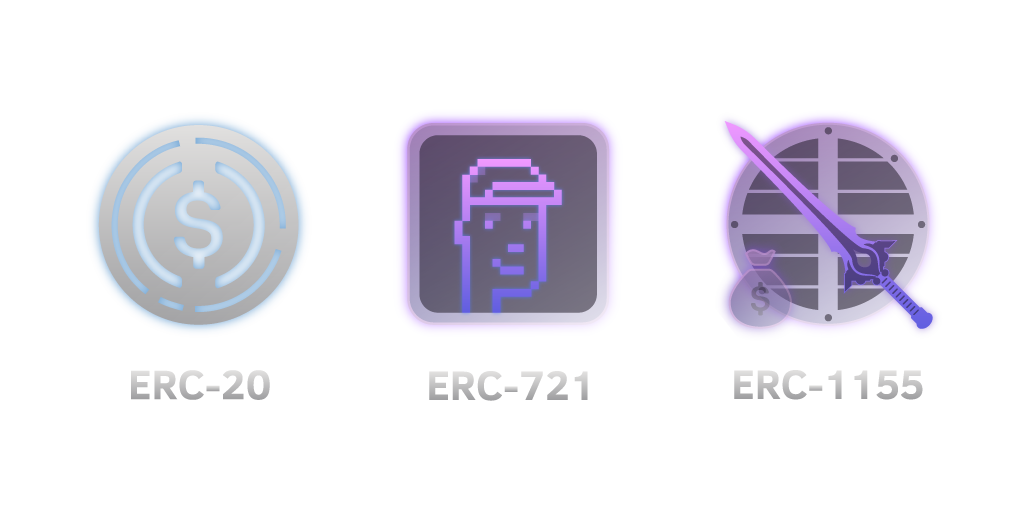
\includegraphics[width=\textwidth*2/3]{Token standards.png}
    \centering
    \caption[Token standards]{Token standards. Extracted from ...}
    \label{fig:token_standards}
\end{figure}

In a more detailed explanation for each of these standards:

\paragraph{ERC-20 (Ethereum Request for Comment 20):}
ERC-20 is the most commonly used token standard on the Ethereum blockchain,
governing the creation and implementation of fungible tokens. These tokens are
interchangeable and have identical properties, allowing them to be traded on
cryptocurrency exchanges seamlessly. ERC-20 tokens adhere to a set of standard
functions, including methods for transferring tokens, querying token balances,
and approving token transfers on behalf of other addresses. Many of the initial
coin offerings (ICOs), token sales, and decentralized finance (DeFi) projects
on Ethereum utilize ERC-20 tokens due to their widespread adoption and
compatibility with Ethereum wallets and exchanges.

\paragraph{ERC-721 (Ethereum Request for Comment 721):}
ERC-721 is a token standard on the Ethereum blockchain that governs the
creation and implementation of non-fungible tokens (NFTs). Unlike ERC-20
tokens, each ERC-721 token is unique and indivisible, representing ownership or
proof of authenticity of a specific asset. ERC-721 tokens are commonly used to
represent digital assets such as digital art, collectibles, virtual real
estate, and in-game items. Each token is assigned a unique identifier (token
ID), allowing it to be distinguished from other tokens within the same
contract. The ERC-721 standard defines methods for transferring tokens,
querying token ownership, and managing metadata associated with each token,
enabling a wide range of use cases in the burgeoning NFT market.

\paragraph{ERC-1155 (Ethereum Request for Comment 1155):}
ERC-1155 is a token standard on the Ethereum blockchain that supports the
creation and management of both fungible and non-fungible tokens within the
same contract. This allows developers to efficiently manage multiple token
types and reduce gas costs associated with deploying multiple contracts.
ERC-1155 tokens are highly flexible and versatile, making them suitable for a
wide range of applications, including gaming, digital collectibles, and
decentralized finance (DeFi). They provide developers with the ability to
create tokenized assets with varying degrees of uniqueness and scarcity. The
ERC-1155 standard defines methods for transferring tokens, querying token
balances, and managing batch transfers of multiple token types, offering
enhanced functionality compared to previous token standards.

These token standards represent just a few examples of the diverse range of
standards shaping the landscape of tokenization on blockchain networks. As
blockchain technology continues to evolve, new standards are likely to emerge,
offering innovative solutions and driving further adoption of digital tokens
across various industries.

\subsection{Non-Fungible Tokens (NFTs)}
\label{subsec:nfts}

Since we're talking about a ticketing system for events, we can see a lot of
potential in the use of NFTs to represent digital tickets, providing a secure
and verifiable means of ticket issuance, transfer, and validation. NFT-based
tickets can be associated with unique metadata, such as event details, seat
numbers, and access permissions, providing a rich and customizable ticketing
experience for event organizers and attendees. NFTs can also be used to create
limited edition or VIP tickets, offering exclusive access and additional
benefits to holders of these special tickets.
